\documentclass{standalone}% For the example only, any class will do
\usepackage{tikz}

\begin{document}



\tikzset{every picture/.style={line width=0.75pt}} %set default line width to 0.75pt

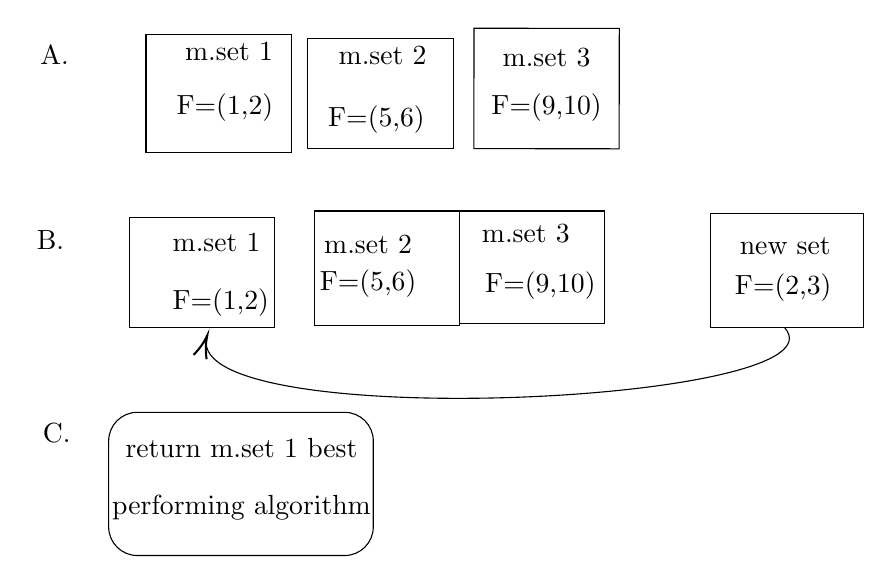
\begin{tikzpicture}[x=0.75pt,y=0.75pt,yscale=-1,xscale=1]
%uncomment if require: \path (0,300); %set diagram left start at 0, and has height of 300

%Shape: Rectangle [id:dp7517769209241454]
\draw   (84,20) -- (154,20) -- (154,77) -- (84,77) -- cycle ;
%Shape: Rectangle [id:dp9115248835353136]
\draw   (162,22) -- (232,22) -- (232,75) -- (162,75) -- cycle ;
%Shape: Rectangle [id:dp5619634747899049]
\draw   (242.03,16.95) -- (312.03,17.05) -- (311.94,75.05) -- (241.94,74.95) -- cycle ;
%Shape: Rectangle [id:dp7066202621172746]
\draw   (356,106) -- (429.5,106) -- (429.5,161) -- (356,161) -- cycle ;
%Shape: Rectangle [id:dp07658366281244189]
\draw   (165,105) -- (235,105) -- (235,160) -- (165,160) -- cycle ;
%Shape: Rectangle [id:dp8045419476810178]
\draw   (235,105) -- (305,105) -- (305,159) -- (235,159) -- cycle ;
%Shape: Rectangle [id:dp5585660554036409]
\draw   (76,108) -- (146,108) -- (146,161) -- (76,161) -- cycle ;
%Curve Lines [id:da6765581083352479]
\draw    (391.5,161) .. controls (425.16,197.63) and (104.02,212.7) .. (113.12,166.42) ;
\draw [shift={(113.5,165)}, rotate = 468.43] [color={rgb, 255:red, 0; green, 0; blue, 0 }  ][line width=0.75]    (10.93,-3.29) .. controls (6.95,-1.4) and (3.31,-0.3) .. (0,0) .. controls (3.31,0.3) and (6.95,1.4) .. (10.93,3.29)   ;

%Rounded Rect [id:dp17433006195713507]
\draw   (66,215.8) .. controls (66,208.18) and (72.18,202) .. (79.8,202) -- (179.7,202) .. controls (187.32,202) and (193.5,208.18) .. (193.5,215.8) -- (193.5,257.2) .. controls (193.5,264.82) and (187.32,271) .. (179.7,271) -- (79.8,271) .. controls (72.18,271) and (66,264.82) .. (66,257.2) -- cycle ;

% Text Node
\draw (124,28) node  [align=left] {m.set 1};
% Text Node
\draw (122,55) node  [align=left] {F=(1,2)};
% Text Node
\draw (195,61) node  [align=left] {F=(5,6)};
% Text Node
\draw (277,55) node  [align=left] {F=(9,10)};
% Text Node
\draw (198,30) node  [align=left] {m.set 2};
% Text Node
\draw (277,31) node  [align=left] {m.set 3};
% Text Node
\draw (40,30) node  [align=left] {A.};
% Text Node
\draw (38,119) node  [align=left] {B.};
% Text Node
\draw (41,212) node  [align=left] {C.};
% Text Node
\draw (118,120) node  [align=left] {m.set 1};
% Text Node
\draw (120,149) node  [align=left] {F=(1,2)};
% Text Node
\draw (191,121) node  [align=left] {m.set 2};
% Text Node
\draw (191,140) node  [align=left] {F=(5,6)};
% Text Node
\draw (267,116) node  [align=left] {m.set 3};
% Text Node
\draw (274,141) node  [align=left] {F=(9,10)};
% Text Node
\draw (392,122) node  [align=left] {new set};
% Text Node
\draw (391,142) node  [align=left] {F=(2,3)};
% Text Node
\draw (130,219) node  [align=left] {return m.set 1 best};
% Text Node
\draw (130,248) node  [align=left] {performing algorithm};


\end{tikzpicture}
\end{document}
